\documentclass[]{book}
\usepackage{lmodern}
\usepackage{amssymb,amsmath}
\usepackage{ifxetex,ifluatex}
\usepackage{fixltx2e} % provides \textsubscript
\ifnum 0\ifxetex 1\fi\ifluatex 1\fi=0 % if pdftex
  \usepackage[T1]{fontenc}
  \usepackage[utf8]{inputenc}
\else % if luatex or xelatex
  \ifxetex
    \usepackage{mathspec}
  \else
    \usepackage{fontspec}
  \fi
  \defaultfontfeatures{Ligatures=TeX,Scale=MatchLowercase}
\fi
% use upquote if available, for straight quotes in verbatim environments
\IfFileExists{upquote.sty}{\usepackage{upquote}}{}
% use microtype if available
\IfFileExists{microtype.sty}{%
\usepackage{microtype}
\UseMicrotypeSet[protrusion]{basicmath} % disable protrusion for tt fonts
}{}
\usepackage[b5paper,tmargin=1.5cm,bmargin=1.5cm,lmargin=1.5cm,rmargin=1.5cm]{geometry}
\usepackage{hyperref}
\PassOptionsToPackage{usenames,dvipsnames}{color} % color is loaded by hyperref
\hypersetup{unicode=true,
            pdftitle={Intelligent Transportation Systems ITS - II},
            pdfauthor={Andres Ladino - Angelo Furno},
            colorlinks=true,
            linkcolor=Maroon,
            citecolor=Blue,
            urlcolor=Blue,
            breaklinks=true}
\urlstyle{same}  % don't use monospace font for urls
\usepackage[style=nature]{biblatex}

\addbibresource{book.bib}
\usepackage{color}
\usepackage{fancyvrb}
\newcommand{\VerbBar}{|}
\newcommand{\VERB}{\Verb[commandchars=\\\{\}]}
\DefineVerbatimEnvironment{Highlighting}{Verbatim}{commandchars=\\\{\}}
% Add ',fontsize=\small' for more characters per line
\usepackage{framed}
\definecolor{shadecolor}{RGB}{248,248,248}
\newenvironment{Shaded}{\begin{snugshade}}{\end{snugshade}}
\newcommand{\AlertTok}[1]{\textcolor[rgb]{0.94,0.16,0.16}{#1}}
\newcommand{\AnnotationTok}[1]{\textcolor[rgb]{0.56,0.35,0.01}{\textbf{\textit{#1}}}}
\newcommand{\AttributeTok}[1]{\textcolor[rgb]{0.77,0.63,0.00}{#1}}
\newcommand{\BaseNTok}[1]{\textcolor[rgb]{0.00,0.00,0.81}{#1}}
\newcommand{\BuiltInTok}[1]{#1}
\newcommand{\CharTok}[1]{\textcolor[rgb]{0.31,0.60,0.02}{#1}}
\newcommand{\CommentTok}[1]{\textcolor[rgb]{0.56,0.35,0.01}{\textit{#1}}}
\newcommand{\CommentVarTok}[1]{\textcolor[rgb]{0.56,0.35,0.01}{\textbf{\textit{#1}}}}
\newcommand{\ConstantTok}[1]{\textcolor[rgb]{0.00,0.00,0.00}{#1}}
\newcommand{\ControlFlowTok}[1]{\textcolor[rgb]{0.13,0.29,0.53}{\textbf{#1}}}
\newcommand{\DataTypeTok}[1]{\textcolor[rgb]{0.13,0.29,0.53}{#1}}
\newcommand{\DecValTok}[1]{\textcolor[rgb]{0.00,0.00,0.81}{#1}}
\newcommand{\DocumentationTok}[1]{\textcolor[rgb]{0.56,0.35,0.01}{\textbf{\textit{#1}}}}
\newcommand{\ErrorTok}[1]{\textcolor[rgb]{0.64,0.00,0.00}{\textbf{#1}}}
\newcommand{\ExtensionTok}[1]{#1}
\newcommand{\FloatTok}[1]{\textcolor[rgb]{0.00,0.00,0.81}{#1}}
\newcommand{\FunctionTok}[1]{\textcolor[rgb]{0.00,0.00,0.00}{#1}}
\newcommand{\ImportTok}[1]{#1}
\newcommand{\InformationTok}[1]{\textcolor[rgb]{0.56,0.35,0.01}{\textbf{\textit{#1}}}}
\newcommand{\KeywordTok}[1]{\textcolor[rgb]{0.13,0.29,0.53}{\textbf{#1}}}
\newcommand{\NormalTok}[1]{#1}
\newcommand{\OperatorTok}[1]{\textcolor[rgb]{0.81,0.36,0.00}{\textbf{#1}}}
\newcommand{\OtherTok}[1]{\textcolor[rgb]{0.56,0.35,0.01}{#1}}
\newcommand{\PreprocessorTok}[1]{\textcolor[rgb]{0.56,0.35,0.01}{\textit{#1}}}
\newcommand{\RegionMarkerTok}[1]{#1}
\newcommand{\SpecialCharTok}[1]{\textcolor[rgb]{0.00,0.00,0.00}{#1}}
\newcommand{\SpecialStringTok}[1]{\textcolor[rgb]{0.31,0.60,0.02}{#1}}
\newcommand{\StringTok}[1]{\textcolor[rgb]{0.31,0.60,0.02}{#1}}
\newcommand{\VariableTok}[1]{\textcolor[rgb]{0.00,0.00,0.00}{#1}}
\newcommand{\VerbatimStringTok}[1]{\textcolor[rgb]{0.31,0.60,0.02}{#1}}
\newcommand{\WarningTok}[1]{\textcolor[rgb]{0.56,0.35,0.01}{\textbf{\textit{#1}}}}
\usepackage{longtable,booktabs}
\usepackage{graphicx,grffile}
\makeatletter
\def\maxwidth{\ifdim\Gin@nat@width>\linewidth\linewidth\else\Gin@nat@width\fi}
\def\maxheight{\ifdim\Gin@nat@height>\textheight\textheight\else\Gin@nat@height\fi}
\makeatother
% Scale images if necessary, so that they will not overflow the page
% margins by default, and it is still possible to overwrite the defaults
% using explicit options in \includegraphics[width, height, ...]{}
\setkeys{Gin}{width=\maxwidth,height=\maxheight,keepaspectratio}
\IfFileExists{parskip.sty}{%
\usepackage{parskip}
}{% else
\setlength{\parindent}{0pt}
\setlength{\parskip}{6pt plus 2pt minus 1pt}
}
\setlength{\emergencystretch}{3em}  % prevent overfull lines
\providecommand{\tightlist}{%
  \setlength{\itemsep}{0pt}\setlength{\parskip}{0pt}}
\setcounter{secnumdepth}{5}
% Redefines (sub)paragraphs to behave more like sections
\ifx\paragraph\undefined\else
\let\oldparagraph\paragraph
\renewcommand{\paragraph}[1]{\oldparagraph{#1}\mbox{}}
\fi
\ifx\subparagraph\undefined\else
\let\oldsubparagraph\subparagraph
\renewcommand{\subparagraph}[1]{\oldsubparagraph{#1}\mbox{}}
\fi

%%% Use protect on footnotes to avoid problems with footnotes in titles
\let\rmarkdownfootnote\footnote%
\def\footnote{\protect\rmarkdownfootnote}

%%% Change title format to be more compact
\usepackage{titling}

% Create subtitle command for use in maketitle
\newcommand{\subtitle}[1]{
  \posttitle{
    \begin{center}\large#1\end{center}
    }
}

\setlength{\droptitle}{-2em}

  \title{Intelligent Transportation Systems ITS - II}
    \pretitle{\vspace{\droptitle}\centering\huge}
  \posttitle{\par}
    \author{Andres Ladino - Angelo Furno}
    \preauthor{\centering\large\emph}
  \postauthor{\par}
      \predate{\centering\large\emph}
  \postdate{\par}
    \date{10/30/2018}

\usepackage[utf8]{inputenc} % Accent inputs
\usepackage[english]{babel} % English language/hyphenation
\usepackage[T1]{fontenc} % Font encoding
\usepackage{microtype} % Rendering
\usepackage{xspace} % Space optimization
\usepackage{fourier}
\usepackage{booktabs}
\usepackage{amsthm}
\makeatletter
\def\thm@space@setup{%
  \thm@preskip=8pt plus 2pt minus 4pt
  \thm@postskip=\thm@preskip
}
\makeatother

\usepackage{amsthm}
\newtheorem{theorem}{Theorem}[chapter]
\newtheorem{lemma}{Lemma}[chapter]
\theoremstyle{definition}
\newtheorem{definition}{Definition}[chapter]
\newtheorem{corollary}{Corollary}[chapter]
\newtheorem{proposition}{Proposition}[chapter]
\theoremstyle{definition}
\newtheorem{example}{Example}[chapter]
\theoremstyle{definition}
\newtheorem{exercise}{Exercise}[chapter]
\theoremstyle{remark}
\newtheorem*{remark}{Remark}
\newtheorem*{solution}{Solution}
\begin{document}
\maketitle

{
\hypersetup{linkcolor=black}
\setcounter{tocdepth}{1}
\tableofcontents
}
\hypertarget{its-for-smart-mobility}{%
\chapter*{ITS for Smart Mobility}\label{its-for-smart-mobility}}
\addcontentsline{toc}{chapter}{ITS for Smart Mobility}




\begin{figure}

{\centering 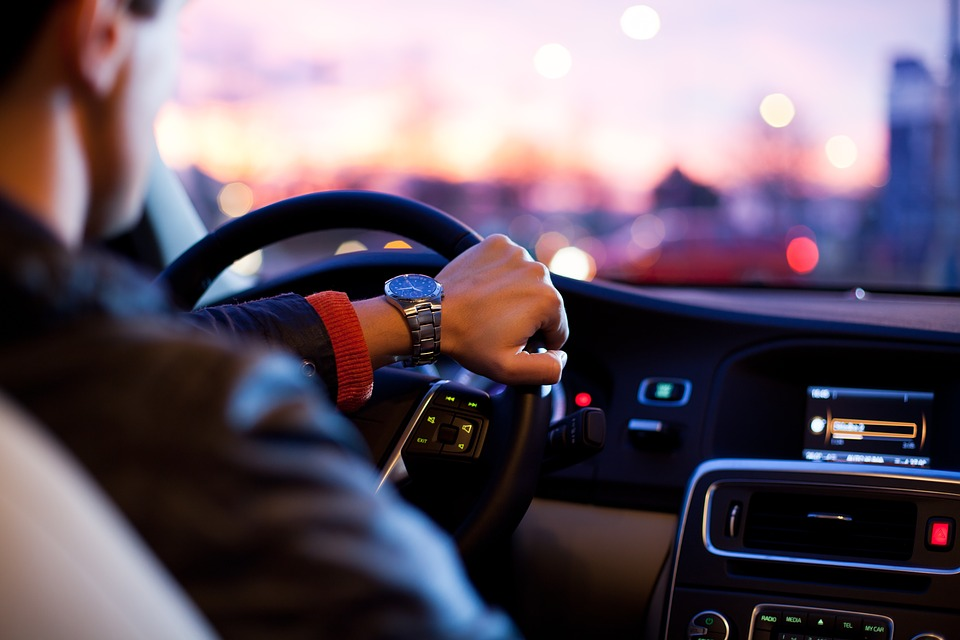
\includegraphics{images/01-car} 

}

\caption{New connected vehicles
\href{Taken\%20from:\%20https://pixabay.com}{https://pixabay.com}.}\label{fig:car}
\end{figure}

\hypertarget{context}{%
\section*{Context}\label{context}}
\addcontentsline{toc}{section}{Context}

Traffic congestion on urban roads is a problem of great interest
nowadays since it strongly affects security and pollution. Workfoce
centralization, population and economic growth alongside with continuous
urbanization are the main causes of traffic congestion. As cities strive
to update/expand the current infrastructures the development of
Information Technologies bring new possiblities as an alternative
solution for transportation systems.

The current project aims to explore some of the new technologies used in
the so called Intelligent Transportation Systems (ITS). They objective
is to study to a certain level of detail some of the new traffic
management systems that will conduct new ways of transportation in the
XXI century. The general idea is based on the fact that information
collected by sensors within traffic networks or in-vehicles sensors can
collect information regarding the traffic condition, perform estimation
of unknown traffic states and decide on specific actions to modify this
state.

Specially, in this case the project will be focused in four main
activities:

\begin{itemize}
\tightlist
\item
  \textbf{Trafic signal design:} This projects aims to study how to
  optimally deal with the design of light cycles to optimize the traffic
  performance. Based on information collected by infrastructure based
  sensors the traffic state can be determined and specific decisions in
  terms on green/red light times can be dynamically adapted.
\item
  \textbf{Connected \& automated vehicles:} New in-vechicle sensors
  create situations in which vehicles may exchange information to
  improve traffic conditions. This project aims to study control
  algorithms implemented in the V2V (Vehicle-vehicle) communication
  layer that can be used to design traffic decisions.
\item
  \textbf{Eco-driving:} Connectivity between vehicles and
  infrastructures will define future directions in transportation.
  Shared information in the V2I (Vehicle-infrastructure) I2V
  (Infrastructure-vehicle) communication layers can optimize traffic
  conditions in apects like fuel-efficiency.\\
\item
  \textbf{Traffic variable reconstruction:} Sensors installed in traffic
  infrastructures provide information regarding the traffic state.
  Nevertheless the solution is not scalable to cover large cities due to
  the economical leverage required to deploy this technology. Algorithms
  to reconstruct traffic information may provide a promising future for
  accurately determine the traffic state of a city. The aim of this
  project is to study how multiple sources of information can be
  integrated to reconstruct traffic variables within a city.
\end{itemize}

\hypertarget{general-objectives}{%
\section*{General Objectives}\label{general-objectives}}
\addcontentsline{toc}{section}{General Objectives}

\begin{itemize}
\tightlist
\item
  Identify new technologies implemented in the Intelligent Transporation
  Systems and investigate how these technologies are deployed in real
  systems.
\item
  Define and determine adequate models that are suitable for deploying
  new ITS technologies.
\item
  Develop specific solutions for ITS that can be tested under
  pre-defined scenarios.
\end{itemize}

\hypertarget{project-information}{%
\chapter{Project information}\label{project-information}}

\hypertarget{deliverables}{%
\section*{Deliverables}\label{deliverables}}
\addcontentsline{toc}{section}{Deliverables}

The project is mainly composed in 3 phases.

\begin{enumerate}
\def\labelenumi{\arabic{enumi}.}
\item
  \textbf{Problem identification \& literature review:} This phases
  consists in:

  \begin{enumerate}
  \def\labelenumii{\arabic{enumii}.}
  \item
    Identify particularly the problem under study, meaning the system to
    be controlled and the way it is assesed.
  \item
    Retrieve bibliographical information about the problem under study.
  \item
    Summarize the already proposed alternatives in the existing
    literature.
  \end{enumerate}

  The main objective of this phase is to understand what are the main
  challenges when solving the specific project under study and to
  present in general ways how this problem has been solved.
\item
  \textbf{Setting up a suitable model:} Once the problem has been
  identified the main objective is to precisely describe the traffic
  models that are suitable for the approach. For this phase the stages
  are divided as:

  \begin{enumerate}
  \def\labelenumii{\arabic{enumii}.}
  \tightlist
  \item
    Determine a specific traffic model that can be used for the
    corresponding situation
  \item
    Define the scenario in which the solution should be tested
  \item
    Pre establish parameters and requirements for the solution to be
    implemented.
  \end{enumerate}
\item
  \textbf{Experimental results:} Finally, the main objective is to
  perform a validation and solution for the problem under study. Several
  tools are provided for this purpose like micro/macro
\end{enumerate}

\begin{center}\rule{0.5\linewidth}{\linethickness}\end{center}

\hypertarget{reporting}{%
\section*{Reporting}\label{reporting}}
\addcontentsline{toc}{section}{Reporting}

In order to fullfill the requirements for each phase each group should
provide a report as follows:

\begin{itemize}
\item
  \emph{Report 1:} Summarizes the results of the 1. Problem
  identification \& literature review and 2. Setting up a suitable
  model. (\textbf{\emph{Due date: January 9th, 2018}})
\item
  \emph{Report 2:} Summarizes the results of the phase 3.Experimental
  results (\textbf{\emph{Due date: January 23rd, 2019}})
\end{itemize}

\hypertarget{project-1-signalized-traffic}{%
\chapter{Project 1: Signalized
Traffic}\label{project-1-signalized-traffic}}

The main objective of this project is to design \emph{traffic light
signal} controls in order to optimize particular traffic conditions.
Traffic signals regularly pre-establish fixed values \emph{red} or
\emph{green} for a particular intersection. In fact the behavior can be
modeled as:



\begin{figure}

{\centering 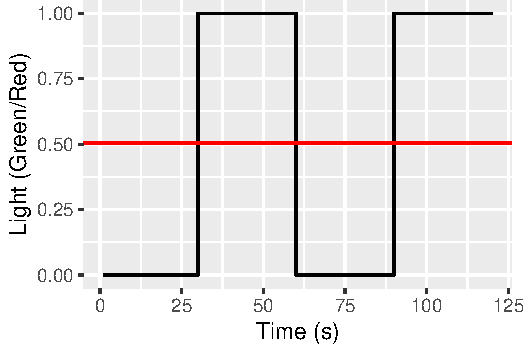
\includegraphics{its-2-project_files/figure-latex/tlight-1} 

}

\caption{Traffic light signal example.}\label{fig:tlight}
\end{figure}

The relationship between the switched green/red time in a traffic light
can be represented by a pulse signal (Figure \ref{fig:tlight}). The red
line in the figure represents the \emph{duty cycle} which represents the
fraction of time the light was in green (\(1\)) with respect to the
total cycle time (\(60s\)). In this case, the main objective is to study
traffic models that can model signalized intersections and design
control laws to design.

\begin{center}\rule{0.5\linewidth}{\linethickness}\end{center}

\hypertarget{objectives}{%
\section*{Objectives}\label{objectives}}
\addcontentsline{toc}{section}{Objectives}

The main objective of this project is to:

\hypertarget{description}{%
\section*{Description}\label{description}}
\addcontentsline{toc}{section}{Description}

\hypertarget{sources}{%
\section*{Sources}\label{sources}}
\addcontentsline{toc}{section}{Sources}

For more details on the project please check:

\begin{itemize}
\item
  \href{https://github.com/andres-ladino-ifsttar/traffic-macrosimulator}{Traffic
  Macrosimulator - Github}
\item
  Check \autocite{Grandinetti2015} available
  \href{https://hal.archives-ouvertes.fr/hal-01188535}{Link} and
  \autocite{Grandinetti2016}
  \href{https://hal.archives-ouvertes.fr/hal-01188811}{Link}
\end{itemize}

\hypertarget{project-2-vehicle-platooning}{%
\chapter{Project 2: Vehicle
Platooning}\label{project-2-vehicle-platooning}}

\hypertarget{objectives-1}{%
\section*{Objectives}\label{objectives-1}}
\addcontentsline{toc}{section}{Objectives}

This project consists in works based on \autocite{Grandinetti2015}

\hypertarget{description-1}{%
\section*{Description}\label{description-1}}
\addcontentsline{toc}{section}{Description}

\hypertarget{sources-1}{%
\section*{Sources}\label{sources-1}}
\addcontentsline{toc}{section}{Sources}

The main reference for this work \autocite{Duret2019}

\hypertarget{project-3-connected-vehicles}{%
\chapter{Project 3: Connected
Vehicles}\label{project-3-connected-vehicles}}

\hypertarget{objectives-2}{%
\section*{Objectives}\label{objectives-2}}
\addcontentsline{toc}{section}{Objectives}

This project consists in works based on \autocite{Grandinetti2015}

\hypertarget{description-2}{%
\section*{Description}\label{description-2}}
\addcontentsline{toc}{section}{Description}

\hypertarget{sources-2}{%
\section*{Sources}\label{sources-2}}
\addcontentsline{toc}{section}{Sources}

\hypertarget{project-4-density-reconstruction}{%
\chapter{Project 4: Density
Reconstruction}\label{project-4-density-reconstruction}}

\begin{figure}

{\centering 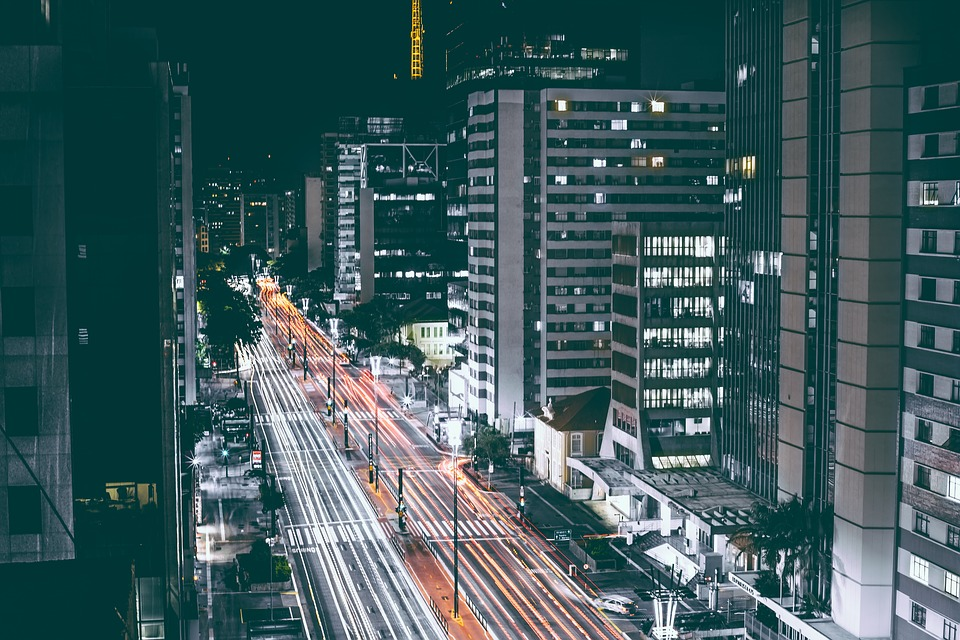
\includegraphics{images/03-density} 

}

\caption{(ref:denres)}\label{fig:denres}
\end{figure}




\begin{Shaded}
\begin{Highlighting}[]
\KeywordTok{plot}\NormalTok{(cars)  }\CommentTok{# a scatterplot}
\end{Highlighting}
\end{Shaded}

\begin{figure}
\centering
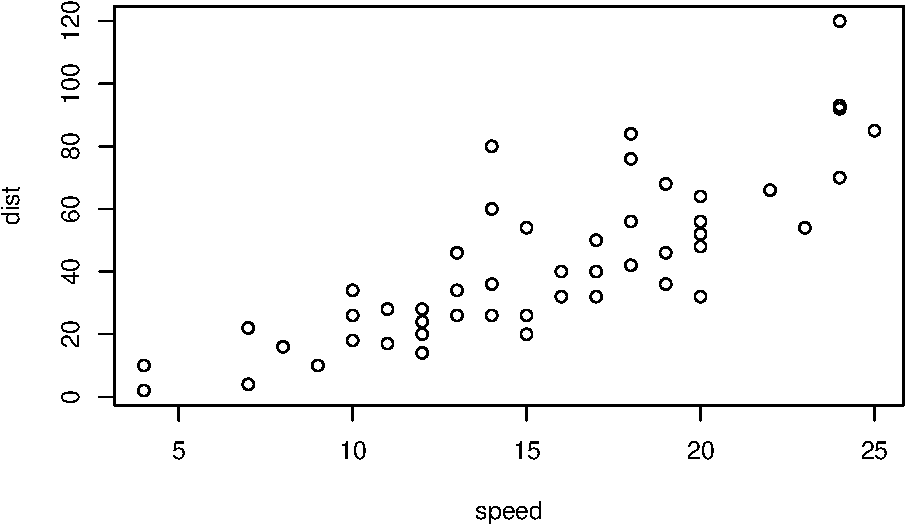
\includegraphics{its-2-project_files/figure-latex/foo-1.pdf}
\caption{\label{fig:foo}A scatterplot of the data \texttt{cars} using \textbf{base} R
graphics.}
\end{figure}

\begin{equation}
f\left(k\right)=\binom{n}{k}p^k\left(1-p\right)^{n-k} \label{eq:binom}
\end{equation}

In \eqref{eq:binom}

Below is an \texttt{align} environment \eqref{eq:align}:

\begin{Shaded}
\begin{Highlighting}[]
\KeywordTok{\textbackslash{}begin}\NormalTok{\{}\ExtensionTok{align}\NormalTok{\}}\SpecialStringTok{ }
\SpecialStringTok{g(X_\{n\}) &= g(}\SpecialCharTok{\textbackslash{}theta}\SpecialStringTok{)+g'(\{}\SpecialCharTok{\textbackslash{}tilde}\SpecialStringTok{\{}\SpecialCharTok{\textbackslash{}theta}\SpecialStringTok{\}\})(X_\{n\}-}\SpecialCharTok{\textbackslash{}theta}\SpecialStringTok{) }\SpecialCharTok{\textbackslash{}notag}\SpecialStringTok{ }\SpecialCharTok{\textbackslash{}\textbackslash{}}
\SpecialCharTok{\textbackslash{}sqrt}\SpecialStringTok{\{n\}[g(X_\{n\})-g(}\SpecialCharTok{\textbackslash{}theta}\SpecialStringTok{)] &= g'}\SpecialCharTok{\textbackslash{}left}\SpecialStringTok{(\{}\SpecialCharTok{\textbackslash{}tilde}\SpecialStringTok{\{}\SpecialCharTok{\textbackslash{}theta}\SpecialStringTok{\}\}}\SpecialCharTok{\textbackslash{}right}\SpecialStringTok{)}
\SpecialStringTok{  }\SpecialCharTok{\textbackslash{}sqrt}\SpecialStringTok{\{n\}[X_\{n\}-}\SpecialCharTok{\textbackslash{}theta}\SpecialStringTok{ ] (}\SpecialCharTok{\textbackslash{}#}\SpecialStringTok{eq:align)}
\KeywordTok{\textbackslash{}end}\NormalTok{\{}\ExtensionTok{align}\NormalTok{\} }
\end{Highlighting}
\end{Shaded}

\begin{align}
g(X_{n}) &= g(\theta)+g'({\tilde{\theta}})(X_{n}-\theta) \notag \\
\sqrt{n}[g(X_{n})-g(\theta)] &= g'\left({\tilde{\theta}}\right)
  \sqrt{n}[X_{n}-\theta ] \label{eq:align}
\end{align}

\hypertarget{sources-3}{%
\section{Sources}\label{sources-3}}

For more details on the project please check:

\begin{itemize}
\tightlist
\item
  \href{https://github.com/aladinoster/density-reconstruction}{Traffic
  Macrosimulator - Github}
\end{itemize}

\hypertarget{reference}{%
\section{Reference}\label{reference}}

The main reference for this project is \autocite{Ladino2018}

\printbibliography


\end{document}
